\documentclass{article}
\usepackage{amssymb,amsmath}
\usepackage{mathtools}
\usepackage{graphicx}
\usepackage{multicol}
\topmargin=-0.3in
\textheight=9.2in
\textwidth=168mm
\oddsidemargin=-0.2in
\evensidemargin=-0.2in

\newcommand{\SLN}{\textit{\textbf{Solution: }}}

\begin{document}
\noindent \textit{\textbf{Steven Rosendahl\\CPSC 330}}
\vspace{2cm}
\begin{enumerate}
\item Assume an instruction cache miss rate for a program is 2\% and a data cache miss rate is 4\%. 
If the processor has a CPI of 2 without any memory stalls and the miss penalty is 100 cycles for all misses, 
determine how much faster a processor would run with a perfect cache that never misses. 
The frequency of all loads and stores is 36\% for SPECint2000.
\begin{quote}
\indent \SLN We want to find the ratio of the performance of the perfect processor over the stalling processor.
We have the following:
\begin{align*}
\frac{\text{Perfect Performance}}{\text{Stall Performance}} &= \frac{\text{CPU Stall}}{\text{CPU Perfect}}\\
&= \frac{\text{Instructions} \times \text{CPI}_{\text{Stall}} \times \text{Clock Cycles}}
{\text{Instructions} \times \text{CPI}_{\text{Perfect}} \times \text{Clock Cycles}}\\ 
&= \frac{\text{CPI}_{\text{Stall}}}{\text{CPI}_{\text{Perfect}}}\\
&= \frac{2 + 2.00 + 1.44}{2}\\
&= 2.72
\end{align*}
\end{quote}
\item Find the AMAT for a processor with a 2ns clock, 
a miss penalty of 20 clock cycles, 
a miss rate of 0.05 misses per instruction, 
and a cache access time (including hit detection) of 1 clock cycle.
Assume that the read and write miss penalties are the same and ignore other write stalls.
\begin{quote}
\indent \SLN We have that the equation for \textit{AMAT} is given by
\[
\text{AMAT} = \text{Hit Time} + \text{Miss Rate} \times \text{Miss Penalty}.
\]
Plugging into the equation gives us
\begin{align*}
\text{AMAT} &= 2ns + 0.05 \times (20 \times 2ns)\\
&= 4ns.
\end{align*}
\end{quote}
\item Suppose we can improve the miss rate to 0.03 missed per reference by doubling the cache size. 
This causes the cache access time to increase to 1.2 clock cycles.
Using AMAT as a metric, determine if this is a good trade off.
\begin{quote}
\indent \SLN In this problem, we need to recompute the AMAT for the new processor and compare it to the result in (2).
The AMAT is again given by
\begin{align*}
\text{AMAT} &= (1.2 \times 2ns) + (0.03 \times 20 \times 2ns)\\
&= 3.6ns.
\end{align*}
This result is less than 4ns, so it is a good trade off.
\end{quote}
\item (a) Compute the size of the cache shown below.
(b) Compute the total number of bits required to implement this cache for the Intrisity FastMATH embedded fast microprocessor 
(this number represents the total amount of memory needed for storing all data, tags, and valid bits).
\begin{center}
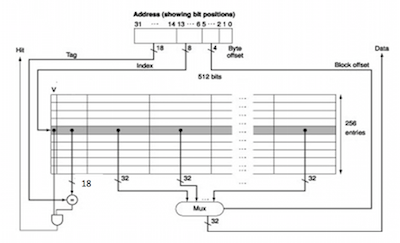
\includegraphics[scale=0.7]{hw5_graphic}
\end{center}
\begin{quote}
\indent \SLN\\
\hspace{3cm} (a) In order to determine the cache size, we need to first determin the number of entries in the cache.
From the diagram, we can see that we have $2^{8}$ entries, or 256 bytes.
Next, we know that there are 16 slots of size 32 bits in each entry in the cache.
We have that
\[
\text{Size} = (0.256)\frac{16\times 32}{8} = 16.384\ kb.
\]
(b) The total number of bytes required will be given by
\[
\text{Size Required} = (1 + 18 + 512)256 = 135936\ bytes.
\]
\end{quote}
\item Describe the general characteristics of a program that would exhibit very little temporal 
and spatial locality with regards to data accesses.
\begin{quote}
\indent \SLN With very little spacial locality, a program would not be able to access contiguous blocks of memory quickly.
This would result in a slower access time for the program. 
With very little temporal locality, the program would need to continually access different blocks of memory over a short
period of time, which would result in a slower program.
\end{quote}
\item Describe the general characteristics of a program that would exhibit very high amounts of temporal locality 
but very little special locality with regards to data accesses.
\begin{quote}
\indent \SLN In this case, the program would not be accessing blocks of memory that are close to each other,
which would cause the program to run slowly. However, the program would be keeping track of the frequently
accessed blocks of memory, which allows for it to run faster than in (5). 
\end{quote}
\item Describe the general characteristics of a program that would exhibit very little temporal locality
but very high amounts of special locality with regards to data accesses.
\begin{quote}
\indent \SLN With very little temporal locality, the program would continually access different blocks of memory
for the same data. 
However, the program would be accessing the same blocks of memory, which would make the program a little faster.
\end{quote}
\item 
Consider a memory hierarchy using one of the three organizations for main memory shown below. 
Assume that the cache block size is 16 words, that the width of organization (b) of the figure is four words, 
and that the number of banks in organization (b) of the figure is four. 
If the main memory latency for a new access is 10 memory bus clock cycles and the transfer time is 1 memory bus clock cycle, 
what are the miss penalties (in clock cycles) for each of these organizations?
\begin{center}
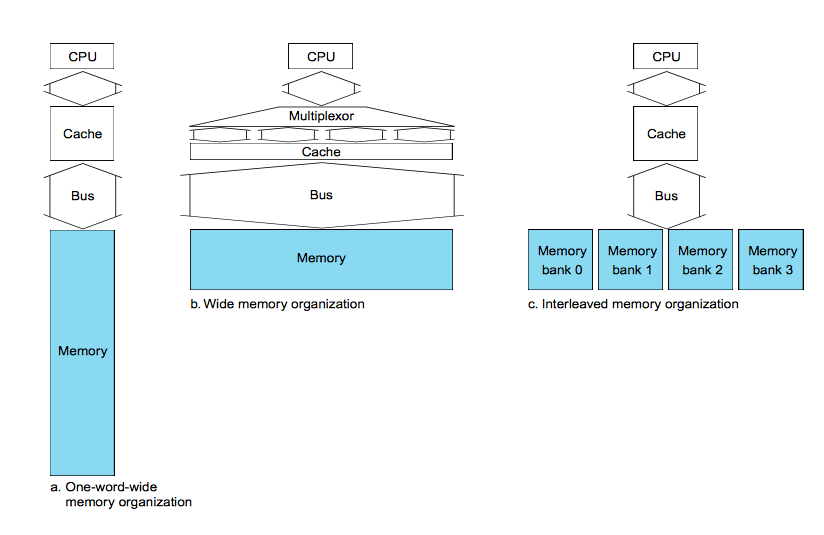
\includegraphics[scale=0.5]{hw5_graphic2}
\end{center}
\begin{quote}
\begin{enumerate}
\item $\text{Miss Penalty} = 1 + 16 \cdot 10 + 16 \cdot 1 = 177$
\item $\text{Miss Penalty} = 1 + 10\cdot\frac{16}{4} + 4\cdot 1 = 45$
\item $\text{Miss Penalty} = 1 + 10\cdot\frac{16}{4} + 16\cdot 1 = 57$
\end{enumerate}
\end{quote}
\item Caches are important to providing a high performance memory hierarchy to processors. 
Given list of 32-bit memory address references given as word addresses: 3,180,43,2,191,88,190,14,181,44,186,253. 
For each of these references, identify the binary address, the tag and the index given in a direct-mapped 
cache with two-word blocks and a total size of 8 bocks. Also, list if each reference is a hit or a miss, 
assuming the cache is initially empty.
\begin{center}
\begin{tabular}{|c|c|c|c|c|}
\hline
Word Address & Binary Address & Tag & Index & Hit/Miss\\
\hline
3 & 0000 0011 & 0 & 1 & Miss\\
\hline
180 & 1011 0100 & 11 & 2 & Miss\\
\hline 
43 & 0010 1011 & 2 & 5 & Miss\\
\hline
2 & 0000 0010 & 0 & 1 & Hit\\
\hline
191 & 1011 1111 & 11 & 7 & Miss\\
\hline
88 & 0101 1000 & 5 & 4 & Miss\\ 
\hline
190 & 1011 1110 & 11 & 7 & Hit\\
\hline
14 & 0000 1110 & 0 & 7 & Miss\\
\hline
181 & 1011 0101 & 11 & 2 & Hit\\
\hline
44 & 0010 1100 & 2 & 6 & Miss\\
\hline
186 & 1011 1010 & 11 & 10 & Miss\\
\hline
253 & 1111 1101 & 15 & 6 & Miss\\
\hline
\end{tabular}
\end{center}
\end{enumerate}
\end{document}